\documentclass[conference]{IEEEtran}
\IEEEoverridecommandlockouts
% The preceding line is only needed to identify funding in the first footnote. If that is unneeded, please comment it out.
\usepackage{cite}
\usepackage{amsmath,amssymb,amsfonts}
\usepackage{algorithmic}
\usepackage{graphicx}
\usepackage{textcomp}
\usepackage{xcolor}
\def\BibTeX{{\rm B\kern-.05em{\sc i\kern-.025em b}\kern-.08em
    T\kern-.1667em\lower.7ex\hbox{E}\kern-.125emX}}

\usepackage{pgfplots}
\usepackage[stdout=false]{pythontex}
% matplotlib2tikz prints messages to stdout, so don't include
% stdout automatically; could also redirect stdout to avoid this
\setpythontexworkingdir{.}
% set PythonTeX to use the document root directory as the working
% directory, so that all plots will be saved there; could use 
% another location, but then would need to specify a path when
% using \input and \InputIfFileExists
    
\newlength\figureheight
\newlength\figurewidth

\usepackage[utf8]{inputenc}
\usepackage[T1]{fontenc}
\usepackage[croatian]{babel}
\begin{document}

\title{Detekcija pakiranih datoteka\\
\thanks{Identify applicable funding agency here. If none, delete this.}
}
\author{\IEEEauthorblockN{Roko Kokan, Jurica Miletić, Ante Sosa}
\IEEEauthorblockA{\textit{Prirodoslovno Matematički fakultet} \\
Zagreb, Hrvatska\\
}
}

\maketitle

\begin{abstract}
Cilj ovog rada je opisati kako detektirati pakirane datoteke uz pomoć alata baziranih na strojnom učenju. Zadatak je osmislila firma ReversingLabs, koja se sama bavi detekcijom malicioznih datoteka. Također, navedena firma nam je dala podatke za treniranje i testiranje našeg modela.
\end{abstract}



\section{Uvod}
Pakiranje je metoda izmjene izvršnih datoteka bez mijenjanja njihove izvorne funkcionalnosti,
ali na način da se datoteka zaštiti od reverznog inženjeringa, da se smanji veličina originalne
izvršne datoteke, ili da se obfuscira maliciozni izvršni kod. Pakiranje podrazumijeva izmjenu
sadržaja datoteke te dodavanje instrukcija koje će prilikom izvršavanja taj sadržaj obnoviti.

Packeri 
modificiraju originalnu izvršnu datoteku na razne načine:
\begin{itemize}
\item Kompresijom podataka
\item Enkripcijom podataka
\item Obfuskacijom
\item Dodavanjem detekcije izvršavanja unutar debuggera ili virtualnog računala
\item Modificiranjem raznih dijelova formata izvršne datoteke
\end{itemize}

U području računalne sigurnosti posebno su učestali packeri za Windows Portable Executable tj. PE datoteke.
PE datoteke su povijesno najčešći nositelji malicioznog koda u 
obliku virusa, ransomwarea, trojanskih konja, itd., te se packeri koriste da bi se taj maliciozni kod prikrio. Klasična statička analiza 
(bez pokretanja datoteka) koju provode antivirusi bazira se na potpisima.
Oni nastaju tako da se prikupe primjeri nekog malwarea te se pronađe niz byteova specifičan za taj malware, 
koji se zatim traži prilikom skeniranja datoteka antivirusom.

Primjenom packera mijenja se sadržaj datoteke, zbog čega potpisi mogu prestati biti prisutni. Na taj se način iz jedne maliciozne datoteke može napraviti više različitih inačica. Packeri koji imaju nemalicioznu primjenu vrlo su rijetki u odnosu na packere koji se koriste za malware. Štoviše, antivirusi često rade potpise za same packere koji se koriste isključivo za malware. Za packere generalne namjene razvijaju se unpackeri kojima se obnavlja originalni sadržaj datoteke za analizu, a detekcija pakiranja nepoznatim formatom snažna je naznaka malwarea.

Ovaj pristup pouzdan je za detekciju pojedinih packera, ali vremenski je zahtjevan čak i za specijalizirane reverzne inžinjere. Osim toga, takav pristup zahtijeva i već izdvojene primjere pakiranih datoteka.

Metoda automatske detekcije pakiranih datoteka omogućuje:
\begin{itemize}
\item Izdvajanje zanimljivih malware datoteka za detaljniju analizu
\item Ranu detekciju nikad prije viđenog malwarea
\item Prepoznavanje malware kampanja 
\end{itemize}


\section{Podaci}
Skup podataka bazirat će se na skupu raznovrsnih packera 
i dodatnim nepakiranim datotekama. Svaki primjer se sastoji 
od dva dijela: originalne datoteke i TitaniumCore izvještaja 
za tu datoteku. 
Cilj zadatka je odvojiti samo pakirane datoteke od 
nepakiranih i raspakiranih, ali će sudionici za razvoj 
modela dobiti detaljnije informacije, poput generalnih 
vrsta packera. U podacima mogu biti varijante višestruko 
pakiranih datoteka, poput dvostruko pakirane datoteke 
koja se tijekom TitaniumCore procesiranja zatim 
jednom raspakira (i dalje se označava kao pakirana).

\section{Problem}
Problem se sastojao od odabira značajki i izgradnje modela stojnog učenja koji će najbolje predvđati jeli dana datoteka pakirana.

\section{Pristup problemu}
Naš pristup problemu bazirao se na pronalaženju glavnih značajki iz TitaniumCore izvještaja.
Značajke koje smo izvukli iz TitaniumCore izvještaja:
\begin{itemize}
\item 10 najčešćih imena odjeljaka (section names) i broj pojavljivanja ostalih odjeljaka
\item 10 najčešćih imena unešenih datoteka (import names)
\item 25 najčešćih programskih sučelja za aplikacije koje koriste izvršne datoteke
\item 25 najčešćih upozorenja koje se javljaju u izvršnim datotekama
\item 16 najčešćih resursa u izvršnim datotekama
\item veličina odjeljaka
\item entropije odjeljaka (ukupna, maksimalna i aritmetička sredina entropija svih odjeljaka)\cite{b1}
\item datum nastanka datoteke
\item imena odjeljaka koji se pojavljuju više od 95\% puta u pakiranim datotekama
\item imena odjeljaka koji se pojavljuju više od 80\% puta u pakiranim datotekama
\item veličina zaglavlja (optional headers)
\end{itemize}
Prvotno smo promatrali samo imena odjeljaka iz čega smo mogli izvući podosta novih značajki. Sama imena odjeljaka mogu biti promjenjena i samim time, ime odjeljka može biti poizvoljno, pa nije baš prepuzdana značajka. Nadalje, promatrali smo koje sve api-je datoteka poziva, iz čega smo pronašli dosta ''sumljivih'' api-ja, te imena datoteka koje su nužne za pokretanje datoteke.  Promatrali smo upozorenja koja se javljaju prilikom izvođenja datoteke, što se nije pokazalo kao najbolja značajka. Također smo veličinu odjeljaka i veličinu cijele datoteke, te smo zaključili, ako je suma veličina svih odjeljaka veća od veličine cijele datoteke, tada je binarni kod datoteke sigurno mijenjaan. 
Značajke vezane za razinu entropije su pokazale kao najpuzdanije. Entropija cijele datoteke, sama kao takva, je previše gruba, ali se u kombinaciji sa entorpijama odjeljaka pokazala kao odlična značajka. Također smo uzeli u obzir minimalnu, maksimalnu i prosječnu vrijednost entropije svih odjeljaka, time smo pokrili slučajeve kada se samo jedan odjeljak promjeni pa je maksimalna entropija odjeljaka povećana.

\begin{figure}[h]
Graf prikazuje broj datoteka u pojedinim skupinama entropije na cijelom skupu koji je primjenjen za treniranje.
\centering
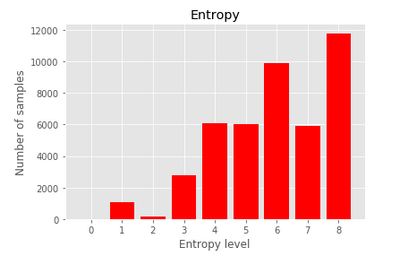
\includegraphics[scale=0.65]{ent.png}
\end{figure}

\begin{figure}[h]
Idući graf prikazuje broj datoteka u pojedinim skupinama maksimalne entropije odjeljaka na cijelom skupu koji je primjenjen za treniranje.
\centering
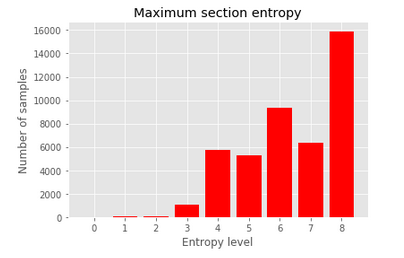
\includegraphics[scale=0.65]{ent5.png}
\end{figure}

Nakon toga smo odlučili analizirati dane značajke izgradnjom modela Random Forest Classifiera i XGBoost treniranjem te bi usporedbom važnosti značajki u jednom od modela zadržali one koje su najviše utjecali na rezultat treniranja danog modela.
\section{Realizacija rješenja}
Prvo smo odlučili istrenirati model XGBoost Classifiera iz biblioteke xgboost u pythonu. Da bismo odredili hiperparametre modela koristili smo Randomized Search CV iz biblioteke sklearn (modul model\_selection) kako bismo pretražili prostor vrijednosti za parametre
\begin{itemize} 
\item max\_depth ( $[1, 2,..., 100]$ )
\item min\_child\_weight ( $[0.1, 0.2,..., 3.0]$ )
\item learning\_rate ( $[0.1, 0.2,..., 3.0]$ )
\item base\_score. ( $[0.5, 0.6, 0.7, 0.8, 0.9] $ )
\end{itemize}
% slika ode kako je prošlo traženje
Nakon toga odabiremo parametre koji daju najbolji rezultat (po srednjoj vrijednosti deseterostruke cross validacije koju provede Randomized Search CV) na nasem skupu podataka za pretraživanje. Također, uz zadane parametre za model xgboosta smo odlučili koristiti 100 stabala (po defaultnim postavkama u XGBClassifieru).
% primjer fitanog modela i njegovog procesa treniranja.
Nakon toga smo odlučili istrenirati model Random Forest Classifier, također određujući hiperparametre modela koristeći Randomized Search CV. Željeli smo pretražiti prostor vrijednosti za parametre 
\begin{itemize} 
\item max\_depth ( $[1, 2,..., 100]$ )
\item criterion ( $[True, False]$ )
\item oob\_score ( $[True, False]$ )
\item max\_features ( $[0.001, 0.002,..., 1.000] $ )
\end{itemize}
% slika ode kako je prošlo traženje
Nakon toga odabiremo parametre na isti način kao i kod XGBClassifiera. Također koristit ćemo 100 stabala (po defaultnim postavkama).
% primjer fitanog modela i njegovog procesa treniranja.
S obzirom na prikazano, XGBoost model nakon treniranja na podacima daje bolje rezultate, te ćemo njega koristiti za daljnju analizu značajki.


Nakon toga odabiremo parametre koji daju najbolji rezultat (po srednjoj vrijednosti deseterostruke cross validacije koju provede Randomized Search CV) na nasem skupu podataka za pretraživanje. Također, uz zadane parametre za model xgboosta smo odlučili koristiti 100 stabala (po defaultnim postavkama u XGBClassifieru).
% primjer fitanog modela i njegovog procesa treniranja.
Nakon toga smo odlučili istrenirati model Random Forest Classifier, također određujući hiperparametre modela koristeći Randomized Search CV. Željeli smo pretražiti prostor vrijednosti za parametre 
\begin{itemize} 
\item max\_depth ( $[1, 2,..., 100]$ )
\item criterion ( $[True, False]$ )
\item oob\_score ( $[True, False]$ )
\item max\_features ( $[0.001, 0.002,..., 1.000] $ )
\end{itemize}
% slika ode kako je prošlo traženje
Nakon toga odabiremo parametre na isti način kao i kod XGBClassifiera. Također koristit ćemo 100 stabala (po defaultnim postavkama).
% primjer fitanog modela i njegovog procesa treniranja.
S obzirom na prikazano, XGBoost model nakon treniranja na podacima daje bolje rezultate, te ćemo njega koristiti za daljnju analizu značajki.
\setlength\figureheight{2.5in}
\setlength\figurewidth{3.5in}
\begin{figure}[h]
\InputIfFileExists{RSXGB.tikz}{}{\textbf{!! Missing graphics !!}}
\caption{Rezultati pretrazivanja parametara sa Random Search CV-om za XGB model}
\end{figure}
\begin{figure}[h]
\InputIfFileExists{XGB_pocetni.tikz}{}{\textbf{!! Missing graphics !!}}
\caption{Rezultati treniranja i validacije modela XGB}
\end{figure}
\begin{figure}[h]
\InputIfFileExists{RSRF.tikz}{}{\textbf{!! Missing graphics !!}}
\caption{Rezultati pretrazivanja parametara sa Random Search CV-om za Random Forest model}
\end{figure}
\begin{figure}[h]
\InputIfFileExists{RandomForest.tikz}{}{\textbf{!! Missing graphics !!}}
\caption{Rezultati treniranja i validacije modela Random Forest}
\end{figure}
\subsection{Analiza značajki}
Nakon što smo istrenirali model na trening podacima, ispisali smo sve značajke, i koju su ulogu one imale pri treniranju XGB modela. 10 najvažnijih značajki u modelu su
\begin{itemize}
\item entropija
	\begin{itemize}
	\item entropy ($15.42289\%$)
	\item mean entropy ($13.67357\%$)
	\item max entropy ($11.02552\%$)
	\item min entropy ($8.93918\%$)
	\end{itemize}
\item import api values ($8.21698\%$)
\item ime odjeljaka
	\begin{itemize}
	\item other sections ($3.12951\%$)
	\item .reloc ($1.36416\%$)
	\item .rdata ($1.63698\%$)
	\end{itemize}
\item import name values ($2.39127\%$)
\item ime importova
	\begin{itemize}
	\item other imports ($1.974\%$)
	\end{itemize}
\end{itemize}
Od sveukupno 113 značajki uzeli smo 30 najznačajnijih, koji imaju utjecaj veći od 0.5\% na treniranje modela, te ćemo njih iskoristiti za treniranje krajnjeg XGBClassifier modela. Opet ćemo provrtjeti Randomized Search CV kako bismo našli najbolje parametre za ovaj podskup značajki.
\begin{figure}[h]
\InputIfFileExists{RSXGBless.tikz}{}{\textbf{!! Missing graphics !!}}
\end{figure}
\section{Zaključak}
Nas krajnji model ima preciznost od 99.08\%. Zakljucili smo da entropija izvrsne datoteke od raznih znacajki koje smo uzeli na promatranje ima najvecu vaznost, te da je pokazala najvecu povezanost sa tim je li izvrsna datoteka pakirana.
\begin{figure}
\InputIfFileExists{Final_model.tikz}{}{\textbf{!! Missing graphics !!}}
\caption{Rezultati cross validacije krajnjeg modela}
\end{figure}
\newpage
\section{Majka}

\begin{thebibliography}{00}
\bibitem{b1} Xabier Ugarte-Pedrero, Igor Santos, Borja Sanz, Carlos Laorden and Pablo Garcia Bringas, ``Countering Entropy Measure Attacks on Packed
Software Detection,'' University of Deusto, Bilbao, Spain.

\end{thebibliography}
\vspace{12pt}
\color{red}
%IEEE conference templates contain guidance text for composing and formatting conference papers. Please ensure that all template text is removed from your conference paper prior to submission to the conference. Failure to remove the template text from your paper may result in your paper not being published.

\end{document}
